% The LaTeX is in here!
\documentclass{article}
\usepackage{graphicx}
\usepackage{ragged2e}
\usepackage{parskip}
\usepackage{float}
\usepackage{hyperref}
\usepackage[utf8]{inputenc}
\setlength{\parindent}{4em}
\usepackage[english]{babel}
\usepackage{geometry}
  \geometry{
    a4paper,
    total={170mm,257mm},
    left=30mm,
    right=30mm,
    top=20mm,
  }
\graphicspath{ {images/} }

\begin{document}
    \begin{center}
    
\includegraphics[scale=0.5]{unb}
    \par
    \vspace{15mm}
    \textbf{Universidade de Brasília - UnB}\\
    \textbf{Instituto de Exatas}\\
    \textbf{Departamento de Ciência da Computação}\\
    \vspace{15mm}
    \textbf{Rodrigo Chaves - 13/0132624}\\
    \textbf{Gabriel Mesquita - 13/0024242}\\
    \vspace{15mm}
    \textbf{Test-drive Development}\\
    \vspace{100mm}
    \textbf{Brasília - DF}\\
    \textbf{2016}
  \end{center}

  \clearpage

  \begin{center}
    Gabriel Mesquita ...\\
    Rodrigo de Araujo Chaves\\
    \vspace{30mm}
    \textbf{Test-driven Development}
    \vspace{30mm}
    \begin{flushright}
      Dissertação sobre por que Test-driven development\\
      é pratica que melhorar a qualidade\\
      final do software apresentanda à disciplina\\
      de Engenharia de Software da Universidade de Brasília.\\
    \end{flushright}
    \vspace{150mm}
    \textbf{Brasília - DF}\\
    \textbf{2016}
  \end{center}

  \clearpage

  \section{Introdução}

  \section{O que é Test-driven Development}

  Test-driven development é um prática de desenvolvimento de software que tem 
  sido usada esporádicamente por decadas. Com essa pratica, um engenheiro de 
  software passo por ciclos entre escrever um teste de unidade que falha e 
  escrevendo a implementação do software para passar nesses testes. 
  Test-driven development tem recentemente resurgindo como uma pratica critica 
  possibilitando metodologias de desenvolvimento ágil de software.

  Quando discutimos sobre TDD, é considerado um conjunto de tarefas requiridas 
  que podem ser implementadas em poucos dias ou menos. Na imagem 1, engenheiros 
  de software produzem código de produção através de rápidas interações como as 
  que seguem:

  \begin{enumerate}
    \item O primeiro passo é adicionar um teste simples o qual é suficiente 
    para a suíte de teste falhar.
    \item Depois executamos nossa suíte para confirmar que os testes realmente 
    estão falhando.
    \item Agora atualize-se o código funcional afim de passar no novo teste.
    \item Executamos a suíte de teste para verificarmos se agora realmente 
    passarmos no novo teste.
    \item Agora com o teste passando: são removidos as duplicações de código 
    afim de limpar o código.
  \end{enumerate}

  \begin{figure}[H]
    \centering
    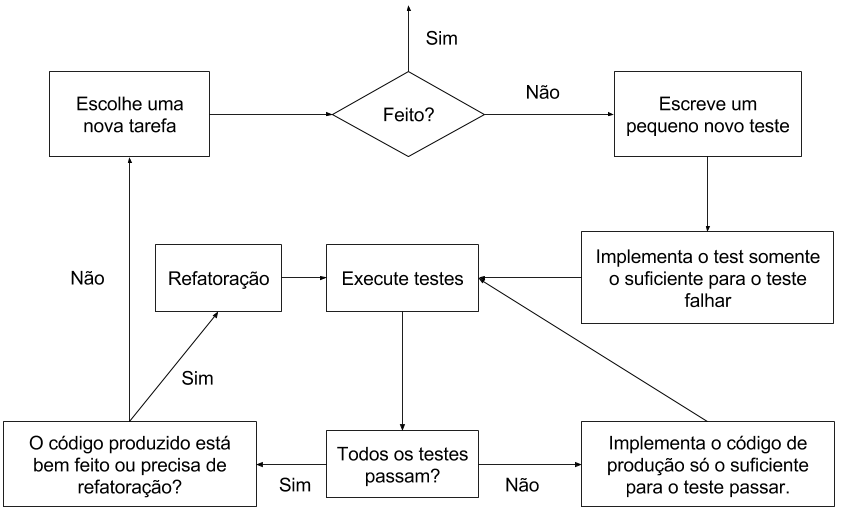
\includegraphics[scale=0.4]{tdd}
    \caption{Fluxograma do TDD}
  \end{figure}

  \section{Design de Software em TDD}

  O Test-driven Development permite que o desenvolvedor que está trabalhando 
  em um módulo pense como serão as responsabilidades, interfaces, serviços os 
  quais serão disponibilizados por esse módulo, enquanto escreve os testes. 
  Depois, quando vai escrever o código de produção, pode se preocupar somente em
  implementar o necessário para passar nos teste já feitos. Fazendo assim, 
  criamos um ritmo entre codificação e teste até que todos os testes criados 
  sejam implementados.

  Pensando no design do projeto, os desenvolvedores do projeto podem criar
  classes e módulos mais coesoes e menos acopladas por que, durante a fase de 
  elaboração dos testes, conseguem visualizar a arquitetura geral da aplicação e
  melhorar como o compenente que irão desenvolver irá conservar com os outros 
  componentes. Em alguns testes, os desenvolvedores os escrevem usando o 
  componente em desenvolvimento como já estivesse pronto e validam se
  esse consegue ser comunicar com suas interfaces.

  Em Test-driven Development, o código desenvolvido é mantido dentro do controle
  intelectual do desenvolvedor, já que o próprio escreveu os testes e ele ou 
  ela está fazendo continuadamente pequenas alterações de design e decisões de 
  implementação, aumentando as funcionalidades do programa em um certo ritmo 
  contínuo.

  \section{Objetivos ao se praticar TDD}

  TDD é uma prática de desenvolvimento que tem por objetivo garantir a
  qualidade e a confiabilidade do produto o mais rápido possível. Ao decorrer do
  desenvolvimento, todo o código elaborado é desenvolvido em conjunto com uma
  suíte de testes automatizados. Esses testes permitem uma segurança maior ao
  desenvolvedor quando precisa mudar algo que já foi implementado ou precisa 
  refotaror o código.

  Além disso, desenvolvedores experientes em TDD podem analisar se os testes 
  produzidos estão difíceis de serem feitos e podem fazer refactoring ou 
  mudanças.

  \section{Referências}

  \begin{flushleft}
  Nachiappan Nagappan, E. Michael Maximilien, Thirumalesh Bhat,
  Laurie Williams, Realizing quality improvement through test driven 
  development: results and experiences of four industrial teams. Disponível em
  \url{http://link.springer.com/article/10.1007/s10664-008-9062-z#/page-1}.
  Acessado em 26 de maio de 2016.

  Andreas Augustin, Test-Driven Development: Concepts, Taxonomy, and Future 
  Direction. Disponível em \url{https://www.semanticscholar.org/paper/Test-
  Driven-Development-Concepts-Taxonomy-and-Janzen-Saiedian/bdcd570eb6a45d7a
  9107a18e25f54b741b92177f/pdf}. Acessado em 26 de maio de 2016

  Martin Fowler, Bill Venners: Test-Driven Development, A Conversation with 
  Martin Fowler. Disponível em \url{http://www.biology.emory.edu/research/Prinz
  /Cengiz/cs540-485-FA12/resources/testDrivenDev.pdf}. Acessado em 30 de maio de
  2016.

  Mauricio Finavaro Aniche, Como a prática de TDD influencia o projeto de 
  classes em sistemas orientados a objetos. Disponível em 
  \url{http://www.teses.usp.br/teses/disponiveis/45/45134/tde-31072012-181230
  /publico/dissertacao.pdf}. Acessado em 30 de maio de 2016.
  \end{flushleft}

\end{document}